\documentclass[../main.tex]{subfiles}

\begin{document}
\section{Detecting and avoiding spectral pollution}
By now, we know our nuisance quite well. We now turn to methods of detecting or avoiding spurious eigenvalues, which is a large focus of research in the area 

This section will mostly stick to heuristic derivations and numerical examples. Proofs are often highly non-trivial, and tend to be worth an entire paper to themselves (e.g. \cite{soussi2006convergence}) or are currently open problems (e.g. \cite{chandler-wilde2012spectrum}).

\subsection{Properties of eigenfunctions}
If there are only a small number of eigenvalues which we would like to learn more about (e.g. once we have whittled down some of the pollution via a dissipative barrier), it may be useful to then look at the eigenfunctions for each relevant value. Polluting eigenvalues have rather interesting-looking eigenfunctions (Figure \ref{fig:TODO})

\subsection{Dissipative barrier methods}\label{sec:dissipative-barrier}
Perhaps one of the simplest methods for separating eigenvalues from spectral pollution is the dissipative barrier method.
This method leverages finite-rank perturbation of an operator.

Take an operator $T$ on a Hilbert space, and
let $P$ be an orthonormal projection onto a finite-dimensional space  such that for an eigenvector $u$, $\|Pu - u\|$ is sufficiently small.
Let $\lambda$ be the eigenvalue for $u$. Then for the operator $T+iP$,

$$(T+iP) u = Tu + iPu \approx \lambda u + iu = (\lambda + i)u.$$

i.e. $(\lambda + i)$ is approximately an eigenvalue for $T+iP$. 

Then, the eigenvalues of the perturbed operator will have imaginary part of approximately 1, and the set of eigenvalues produced by the approximation 
can be filtered to discard points without imaginary part close to 1 as being pollution. This is particularly useful for self-adjoint operators, where the entire spectrum and the essential numerical range are a subset of the real line; in that case, the perturbed eigenvalues will be the only points on the spectrum with significant imaginary part. Even better, if the operator is also bounded, then all pollution is in the essential numerical range (Theorem \ref{}) which is
invariant under compact perturbation (Theorem \ref{}) so the pollution will converge to the real axis.

Let us see this concretely with an example.

\begin{example}
We return once again to our discontinuous multiplication operator $M_f$ on $L^2(0, 1)$ with symbol
$$
f: x \mapsto \begin{cases}
x & x < 1/2\\
x+1/2 & \text{otherwise}.
\end{cases}
$$
This time, we add a `rank-one perturbation' to get the operator $\tilde{M}$ which has the action
$$\tilde{M}u = M_fu + (u, \varphi) \varphi,$$
where $\varphi$ is a real-valued function on $L^2(0, 1)$. Then $\tilde{M}$ has an eigenvector: we rearrange to get
\begin{align*}
f(x)u(x) + (u, \varphi)\varphi(x) & = \lambda u(x),\\
\text{therefore }(\lambda - f(x))u(x) & = (u, \varphi)\varphi(x),\\
u(x) & = c \frac{\varphi(x)}{\lambda - f(x)}
\end{align*}
for some constant $c$. We then normalise this to $\frac{\varphi(x)}{\lambda - f(x)}$, which requires
\begin{align*}
f(x)u + (u, \varphi)\varphi & = \lambda u \\
(f(x) - \lambda)c\frac{\varphi(x)}{\lambda - f(x)} + (\frac{c\varphi}{\lambda - f}, \varphi)\varphi(x) & = 0 \\
-1 + (\frac{\varphi}{\lambda - f}, \varphi) & = 0
\end{align*}
so we can normalise provided that $(\frac{\varphi}{\lambda - f}, \varphi) = \int_0^1 \frac{|\varphi|^2}{\lambda - m} = 1.$
\end{example}

Thus for any value $\lambda$ we can choose $\varphi \in L^2(0, 1)$ and scale it so that $\int_0^1 \frac{|\varphi|^2}{\lambda - m} = 1$
to get an operator $\tilde{M}$ with spectrum $\Spec(M) \cup \{\lambda \in \mathbb{C} : \int_0^1 \frac{|\varphi|^2}{\lambda - m} = 1\}$. In Figure \ref{fig:nodbm} we can see the results of Ritz approximations
with $\varphi$ chosen such that the operator has an eigenvalue at 0.7.\footnote{In particular, $\varphi$ was chosen to be the constant
$(\log(3) - 3\log(2) + \log(5) + \log(7) - \log(10))^{-1}$; this satisfies the normalisation condition at $\lambda = 0.7$ but also at $\lambda \approx 4.4$;
the eigenvalue at $\lambda \approx 4.4$ has been cropped out of the figure to improve illustration of the idea.} In Figure \ref{fig:dbm} we see the same approximation but with the dissipative barrier $iP$ where $P$ is the projection onto $\mathrm{span}\{\phi_n, |n| \leq 25\}$. Note that the spectrum on the line ${(x, y) : \mathrm{Imag}(x) = 1}$ converges to what we'd expect the spectrum to be!

\begin{figure}[p!]
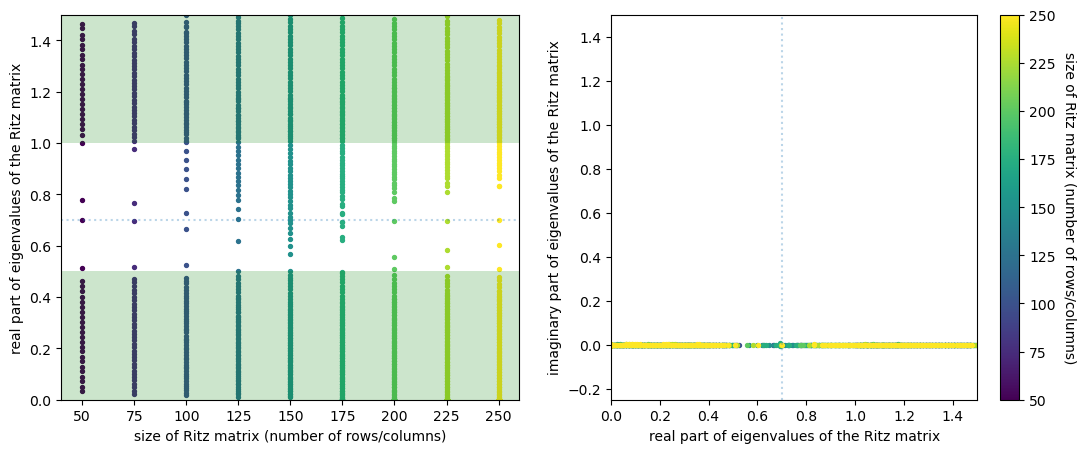
\includegraphics[width=0.9\linewidth, height=6cm]{ptb-mult-nodbm}
\caption{The real part of the approximate spectrum for $\tilde{M}$; on the left, the real parts of the approximate spectrum as the size of the Ritz matrix increases;
on the left, the complex approximate spectrum where colour is used to donate the size of the approximation. The green shaded regions correspond to
the essential spectrum of $\tilde{M}$, and the dotted lines are at $\mathrm{Re}(x) = 0.7$ to show where the added eigenvalue should be. 
(An intuitive way to view these figures is to see them as a three-dimensional plot, with the left figure `top-down', and the right figure `from the east')}
\label{fig:nodbm}
\end{figure}

\begin{figure}[p!]
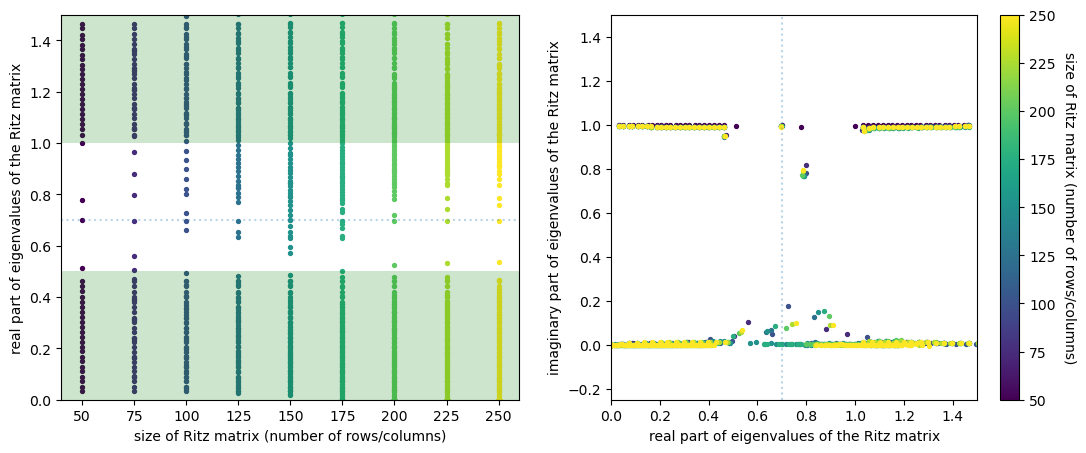
\includegraphics[width=0.9\linewidth, height=6cm]{ptb-mult-dbm} 
\caption{The real part of the approximate spectrum for $\tilde{M}+iP$; compare with Figure \ref{fig:nodbm}. See that the line at 1.0 on the imaginary
axis converges to the actual spectrum of the operator, while the pollution remains below.}
\label{fig:dbm}
\end{figure}
\clearpage

\begin{remark}
One may also note that there are bands corresponding to the essential spectrum with imaginary part 1. 
The reason why dissipative barriers `replicate' the essential spectrum is an open problem; it has recently been investigated specifically for Schr\"odinger operators \cite{stepanenkoTODO} but in general remains unknown.
\end{remark}

As a second example, let us try to replicate some results from Aceto et al. (2006) \cite{aceto2006numerical}. In this paper, they use an algebraic method
combined with a `shooting technique' to find high-accuracy estimates of eigenvalues for a Sturm-Liouville operator; this highly-specialised algorithm
is free from pollution but works only for a specific class of Sturm-Liouville operators.
is a 

\begin{example}\label{ex:aceto}
In particular, take the following eigenvalue problem on $L^2[0, \infty)$:

$$
\begin{cases}
-y'' + (\sin(x) - \frac{40}{1+x^2})y = \lambda y \\
y(0) \cos(\pi/8) + y'(0) \cos(\pi/8) = 0.
\end{cases}
$$

This operator has a `band-gap' structure; it has intervals (bands) of essential spectrum, with eigenvalues dotted in the gaps between bands.
In two of the spectral gaps $J_2 = (-0.34767, 0.59480)$ and $J_3 = (0.91806, 1.2932)$ (denoted in line with the paper and rounded to 5sf) the
algebraic method finds the following eigenvalues:

\begin{figure*}[h!]
\centering
\begin{tabular}{c c}
$J_2$ & $J_3$ \\
\hline\hline
0.33594 & 0.94963 \\
0.53662 & 1.2447 \\
0.58083 & 1.2919 \\
0.59150 & \\
\end{tabular}
\end{figure*}

Firstly, we will see whether we can reproduce this data. The algebraic method used first truncates the half-line to $[0, 70\pi]$. We will do the same and
perform a Ritz approximation on the truncated interval, applying a dissipative barrier; this is a success, as one can see in Figure \ref{fig:aceto-dbm}.

Now we will aim for better; whether we can reproduce these eigenvalues using a Ritz approximation on $[0, \infty)$, with the orthonormal basis $\{\phi_n\}_{n \in \mathbb{N}},
\phi_n = \exp(-x/2)L_n$, where $L_n$ is the n'th Laguerre polynomial (see \cite{szego1975orthogonal} for a proof that this is indeed an orthonormal basis)
\end{example}

\begin{figure}[p!]
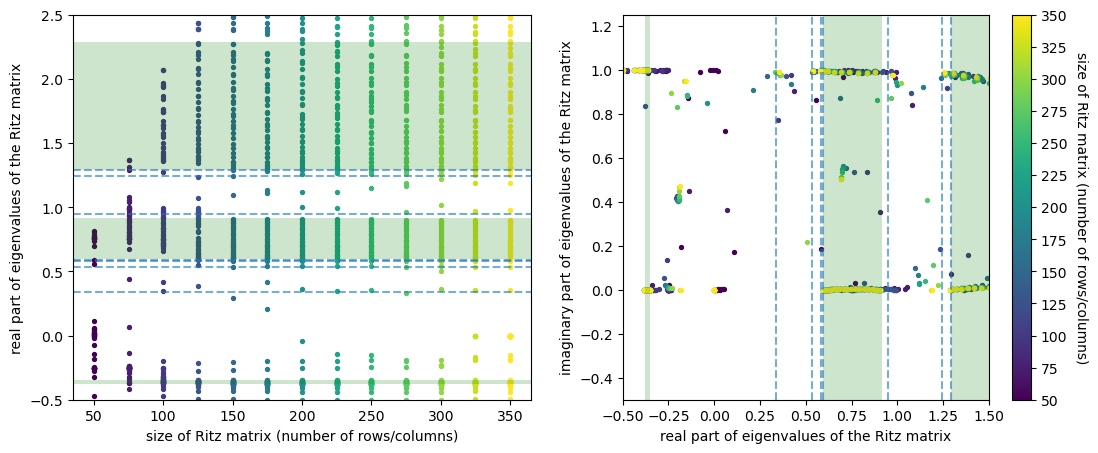
\includegraphics[width=0.9\linewidth, height=6cm]{aceto-dbm}
\caption{The results of truncating the domain and applying a dissipative barrier to the operator of Example \ref{ex:aceto}.
The green bands represent the essential spectrum of the operator, and the dotted blue lines indicate where the algebraic method found
eigenvalues in two spectral gaps. Note that for larger approximations, the points in the spectral gaps with imaginary part 1.0 are
very close to the algebraic method's approximation.}
\label{fig:aceto-dbm}
\end{figure}
\clearpage

\subsection{Floquet theory}
For differential operators with a periodic element (such as Sturm-Liouville operators with periodic potential), their spectral theory is interwoven with Floquet theory, which can simplify the system down to the study of a `fundamental matrix'. A similar theory can be developed for discrete `finite difference' problems - this theory will allow us to \emph{exactly} solve certain problems with a modification of the truncation method.

\begin{definition}{\textbf{(Central finite difference and discrete Laplacian)}}
The central finite difference of a function $u: \mathbb{Z} \rightarrow \mathbb{C}$ is 
$$D_c u (n) = \frac{u(n+1) - u(n-1)}{2}.$$

We can then define the second finite difference, or discrete Laplacian, as $\Delta_c = D_c^2$.
\end{definition}
A natural representation of the function $u: \mathbb{Z} \rightarrow \mathbb{C}$ is as a doubly infinite column vector,
$$u = (\hdots u(-1), u(0), u(1),\hdots)^T.$$
Then we can represent our finite differences as matrix multiplication of $u$ by a doubly infinite matrix, such as

$$ 
D_c = \begin{pmatrix*}[c]
\ddots & \ddots & & & \\
\ddots & 0 & 1 & & \\
& -1 & 0 & 1 & \\
& & -1 & 0 & \ddots \\
& & & \ddots & \ddots \\
\end{pmatrix*}\quad\quad
\Delta_c =
\begin{pmatrix*}[c]
\ddots & \ddots & & & \\
\ddots & -2 & 1 & & \\
& 1 & -2 & 1 & \\
& & 1 & -2 & \ddots \\
& & & \ddots & \ddots \\
\end{pmatrix*}.
$$

These infinite tridiagonal matrices are known as Jacobi matrices. The discrete Laplacian is often transformed into the `free Jacobi matrix' $J_0 = \Delta_c + 2I$, as this simplifies the structure without affecting the spectrum (it only shifts it over by 2). Another example of a Jacobi matrix is the diagonal operator $\diag(q)$ for some $q: \mathbb{Z} \rightarrow \mathbb{C}$, defined as the multiplication operator $\diag(q)v(n) = q(n)v(n)$.

$$
\diag(u) =
\begin{pmatrix*}[c]
\ddots & \ddots & & & \\
\ddots & q_{-1} & 0 & & \\
& 0 & q_0 & 0 & \\
& & 0 & q_1 & \ddots \\
& & & \ddots & \ddots \\
\end{pmatrix*}.
$$

We will use this matrix form as our primary representation of a tridiagonal operator, but using them without our original definition (given in general below) to fall back on raises some issues that must be addressed: if the matrix is doubly infinite, how do we define a `main diagonal'? How do we ensure that our infinite column vectors `line up' correctly with our infinite matrices? (this is a question explored in detail in \cite{lindnerTODO}).
The reader may notice that the finite difference matrices are Toeplitz, and the theory of section \ref{sec:toeplitz} applies to them. However, the diagonal operator is not Toeplitz, and the Jacobi matrix begins to be interesting where it ceases to be (generally) Toeplitz:

\begin{definition}{\textbf{(General second-order finite difference operator)}}
For any set X, let $X^\mathbb{Z}$ be the set of doubly infinite sequences $\mathbb{Z} \rightarrow X$. Consider three sequences: $b_n \in \mathbb{C}^\mathbb{Z}$ and $a_n, c_n \in (\mathbb{C} \setminus 0)^\mathbb{Z}$.\\
A general second-order finite difference operator $J: \mathbb{C}^\mathbb{Z} \rightarrow \mathbb{C}^\mathbb{Z}$ is then defined by the action
\begin{equation}\label{eqn:2efde}
Ju (n) = a_n u(n-1) + b_n u(n) + c_{n+1} u(n+1)
\end{equation}
We will define specific Jacobi operators via the notation $J = J(a_n, b_n, c_n)$ for convenience.
\end{definition}
As one would expect, this is represented as the Jacobi matrix

$$
J =
\begin{pmatrix*}[c]
\ddots & \ddots & & & \\
\ddots & b_{-1} & c_0 & & \\
& a_0 & b_0 & c_1 & \\
& & a_1 & b_1 & \ddots \\
& & & \ddots & \ddots \\
\end{pmatrix*}.
$$

\begin{proposition}\label{thm:2efde-sols}
Given a Jacobi matrix $J$, the initial value problem for some initial points $n_0, n_0 + 1$
$$
\begin{cases}
Ju = f\\
u(n_0) = a\\
u(n_0 + 1) = b
\end{cases}
$$
has a unique solution.
\end{proposition}
\begin{proof}
We can rearrange equation (\ref{eqn:2efde}) to see that $u(n-1)$ is uniquely determined by $u(n)$ and $u(n+1)$, and $u_{n+1}$ by $u(n)$ and $u(n-1)$. This creates a three-term recurrence relation in both directions - thus an entire sequence $u \in \mathbb{C}^\mathbb{Z}$ can be determined from the two initial conditions.
\end{proof}

\begin{proposition}\label{thm:2efde-ker-dim}
The kernel of $J$, $N_0(J) \eqdef \{u \in \mathbb{C}^\mathbb{Z} : Ju = 0\}$ is a two-dimensional subspace of $\mathbb{C}^\mathbb{Z}$; therefore, the eigenspace of $J$, $N_\lambda(J) \eqdef \{u \in \mathbb{C}^\mathbb{Z} : (J - \lambda)u = 0\}$ for any eigenvalue $\lambda$, is also two-dimensional.
\end{proposition}
\begin{proof}
For some Jacobi matrix $J$, define a `solution map' $S: \mathbb{C}^2 \rightarrow \mathbb{C}^2$ which maps pairs of complex numbers $(a, b)$ to the solution of
$$
\begin{cases}
Ju = 0\\
u(0) = a\\
u(1) = b.
\end{cases}
$$
We now show that $S$ is a linear isomorphism from $\mathbb{C}^2$ to the kernel $N_0 (J)$.
\begin{enumerate}[I.]
\item First we show $S$ is linear. Consider $a, b, c, d, e \in \mathbb{C}$, and let $S(a, b) = u$, $S(d, e) = v$.
Then by the linearity of $J$, for $w = cu + v$, $Jw = cJu + Jv = 0$. Then $w$ solves
$$
\begin{cases}
Jw = 0\\
w(0) = ca + d\\
w(1) = cb + e
\end{cases}
$$
which by uniqueness must mean $S(c(a, b) + (d, e)) = w = cS(a, b) + S(d, e)$.

\item The injectivity of $S$ is almost immediate: let $S(a, b) = S(c, d) = u$. Then $u(0) = a$ and $u(0) = c$, therefore $a = c$, and likewise $u(1) = b = d$.

\item Finally, we show that $S$ is surjective. Consider $u \in N_0 (J)$, so $Ju = 0$, and thus it is clear that $u = S(u(0), u(1)).$
\end{enumerate}
Then $S$ is a linear isomorphism, so we have $\mathbb{C}^2 \cong N_0 (J)$, and so $\dim(\mathbb{C}^2) = \dim(N_0 (J)) = 2$.

The similar result for eigenspaces follows as $N_\lambda (J) = N_0 (J - \lambda)$. If $J$ is a Jacobi matrix, so is $J - \lambda$; it is $J$ but with the sequence $(b_n)_{n \in \mathbb{Z}}$ replaced by $(b_n - \lambda)_{n \in \mathbb{Z}}$.
\end{proof}

Now let us consider the case where these sequences are periodic. We call a Jacobi matrix $N$-periodic if the sequences $a_n, b_n, c_n$ are all $N$-periodic.

Now consider an operator $M$, which we shall call the \emph{monodromy operator}, with action $Mu(n) = u(n+N)$. If $u(n)$ is a solution for $Ju = \lambda u$, then so is $v(n) = u(n+N)$; thus we can consider $M(\lambda)$ as an operator on $N_\lambda (J)$. Then by Proposition \ref{thm:2efde-ker-dim}, $M(\lambda)$ is an operator on a two-dimensional space, so can be represented as a $2 \times 2$ matrix with respect to some basis. For simplicity, we can use $S$, the `solution map' from Proposition \ref{thm:2efde-ker-dim}; as linear isomorphisms carry a basis to a basis, the two solutions $u_1 = S(1, 0)$ and $u_2 = S(0, 1)$ are a basis of $N_\lambda (J)$. In this basis we have

$$M(\lambda) =
\begin{pmatrix}
u_1(N) & u_2(N) \\
u_1(N+1) & u_2(N+1)
\end{pmatrix}
$$

In the Floquet theory literature, the eigenvalues and eigenvectors of $M(\lambda)$ are referred to as Floquet multipliers and Floquet solutions respectively. $M(\lambda)$ must have at least one eigenvalue for any $\lambda$, and here is where Floquet theory gets its strength: a Floquet solution $u$ satisfies $Ju = \lambda u$ and also has the additional property that $u(n+N) = zu(n).$
\begin{proposition}{\textbf{(Floquet-Bloch decomposition)}}
Let $J$ be the Jacobi operator $J(a_n, b_n, c_n)$. If column vector $(u(1), u(2), ... u(N))^T$ satisfies
%Let $J$ be an $N$-periodic Jacobi matrix, and let $Ju = \lambda u$ have Floquet solution $u$ and Floquet multiplier $z$. Then the column vector $(u(1), u(2), ... u(N))^T$ satisfies

\begin{equation}\label{eqn:floquet-bloch}
\begin{pmatrix*}[c]
b_1 & c_2 & & & a_1/z\\
a_2 & b_2 & c_3 & & & \\
& a_3 & b_3 & \ddots & & \\
& & \ddots & \ddots & c_N & \\
c_{N+1} z & & & a_N & b_N\\
\end{pmatrix*}
\begin{pmatrix*}
u(1) \\
u(2) \\
\vdots \\
u(N)
\end{pmatrix*}
= \lambda
\begin{pmatrix*}
u(1) \\
u(2) \\
\vdots \\
u(N)
\end{pmatrix*}
\end{equation}
for some $z$, then $\lambda$ is an eigenvalue of $J$, and the extension of $u$ to $\mathbb{C}^\mathbb{Z}$
$$\tilde{u}: n \mapsto
z^{k}u(n - kN) \text{ for } kN < n \leq (k+1)N\text{ for some } k \in \mathbb{Z}
$$
is a Floquet solution of $Ju = \lambda u$ with Floquet multiplier $z$.

\end{proposition}
\begin{proof}
For the infinite problem, we have that $u$ is an eigenvector for $J$ if
$$a_n u(n-1) + b_n u(n) + c_{n+1} u(n+1) = \lambda u(n)$$
so in particular as $u(n + N) = z u(n)$,
\begin{align*}
& \frac{a_1}{z} u(N) + b_1 u(1) + c_2 u(2) = \lambda u(1)\\
\Rightarrow \quad& a_1 \tilde{u}(0) + b_1 \tilde{u}(1) + c_2 \tilde{u}(2) = \lambda u(1), \text{ and } \\
& a_N u(N-1) + b_N u(N) + c_{N+1} z u(1) = \lambda u(N)\\
\Rightarrow \quad& a_N \tilde{u}(N-1) + b_N \tilde{u}(N) + c_{N+1} \tilde{u}(N+1) = \lambda u(N)
\end{align*}
which is exactly the first and last column of (\ref{eqn:floquet-bloch}). For any values of $n$ greater than $N$, say $N + k$ for $k \leq N$
\begin{align*}
a_{N+k} \tilde{u}(N+k-1) + b_{N+k} \tilde{u}(N+k) + c_{N+k+1} \tilde{u}(N+k+1) & = \lambda u(N+k) \\
\Rightarrow \quad z a_{k} u(k-1) + z b_{k} u(k) + z c_{k+1} u(k+1) & = \lambda z u(k)
 \end{align*}
where the $z$'s then cancel out. $a_{N+k} = a_{k}$ and likewise for $b$ and $c$ due to periodicity. A similar argument for values less than 1 will give similar results; for $k \geq N$, repeated application of the procedure will again give the same results for some exponent of $z$. Thus a solution to our finite problem (\ref{eqn:floquet-bloch}) extends to a solution to $Ju = \lambda u$. By construction, our extension is a Floquet solution with mulitplier $z$.
\end{proof}

This is much more computationally tractable; if we calculate the spectrum of 

\subsubsection{The `Ten Martini Problem'}
The `Ten Martini Problem'\footnote{so-called for the prize offered by Mark Kac - who conjectured a stronger form known as the `Dry Ten Martini Problem' - for its solution \cite{simon1982almost}.} is a problem surrounding an operator on $\ell^2(\mathbb{Z})$ arising in quantum physics, known as the \emph{almost Mathieu operator}:

$$H_\omega^{\lambda, \alpha} = u(n+1) + u(n-1) + 2\lambda \cos(2\pi (\omega + n \alpha))u(n)$$

for $\alpha, \omega \in [0, 2\pi]$ and $\lambda > 0$. The conjecture, solved by Avila and Jitomirskaya in 2006 \cite{avila2006ten}, is that if $\alpha$ is irrational, then $\Spec(H_\omega^{\lambda, \alpha})$ is homeomorphic to the Cantor set (a pathological subset of $[0, 1]$ which is compact and uncountably large, but is nowhere dense, totally disconnected, and has measure 0). As we can see, this operator is a second-order finite difference operator. Furthermore, if $\alpha$ is rational, then it is a periodic discrete Schr\"odinger operator:

\subsection{Supercell methods}
For discrete systems with a random element, we can use the Floquet-Bloch decomposition of the previous section to avoid spectral pollution entirely, via an approach first devised for studying defects in materials with crystal structure \cite{nieminen2007supercell}. We will discuss these via a physically motivated example

These methods had been used heuristically by physicists and crystallographers from as early as 19%TODO,
and has been made rigorous in certain cases (e.g. Soussi \cite{soussi2006convergence} for Heimholtz operators where the potential is almost periodic with a compactly supported perturbation); for such a simple idea, the proof is incredibly involved. 

\subsubsection{The Feinberg-Zee random hopping model}
Feinberg and Zee (1999) \cite{feinberg1999nonhermitian} models an unusual behaviour in superconductors via a class of non-self-adjoint and random operators on $\ell^2(\mathbb{Z})$: matrices of the form

$$
A \eqdef \begin{pmatrix*}[c]
\ddots & \ddots & & & & \\
\ddots & 0 & 1 & & & \\
& c_{n-1} & 0 & 1 & & \\
& & c_{n} & 0 & 1 & \\
& & & c_{n+1} & 0 & \ddots \\
& & & & \ddots & \ddots & \\
\end{pmatrix*}
$$

which is the Jacobi operator $J(c_n, 0, 1)$. $c_n$ is a random sequence, where for a fixed value $\sigma \in (0, 1]$, $c_n$ takes values from $\{-\sigma, \sigma\}$ at random, taking value $\sigma$ with probability $p$. For random matrices, it is naturally difficult to discern the entire spectrum (one will often instead derive an `almost sure' spectrum of what will be in the spectrum for almost any $p$) \cite{chandler-wilde2012spectrum}.\\

Note that for a discrete problem, the orthonormal basis of $\ell^2(\mathbb{Z})$ are the column vectors $\phi_n = (\delta_{in})_{i \in \mathbb{Z}}$. As a result, all the Galerkin method is really doing is truncating a doubly infinite matrix to a finite matrix. Now if we consider an eigenvector $u$ to the truncated problem, how does it correspond to the original operator? If we denote the sequence in our truncation as $(c_1, ... c_{n-1})$, then on the infinite matrix, the operator maps the first entry $u_1$ to $c_0 u_0 + u_2$ and the last entry $u_{n-1}$ to $c_{n-2} u_{n-2} + u_{n}$. On the other hand, in our truncation, $u_1$ is mapped to $u_2$, and $u_{n-1}$ to $c_{n-2} u_{n-2}$. In a way, we have artificially imposed a boundary condition on $u$, in this case imposing a Dirichlet boundary that $c_k = 0$ for $k \in \mathbb{Z} \setminus \{1, \hdots, n-1\}$. Is this a valid assumption? Some authors suggest that in certain cases, spectral pollution may be entirely due to a heavy-handed choice of imposed boundary \cite{cances2011periodic}.

The supercell method approximates a random tridiagonal matrix by a periodic one. For our Feinberg-Zee matrix, simply replace the random sequence $c_n$ by a $k$-periodic sequence $n \mapsto c_{((n \bmod k )+ 1)}$.\footnote{One can see how this works for sequences on the (super)diagonal similarly. Note there is no particular relevance to the $+1$; it merely helps bookkeeping by keeping our indexing from $1$ to $k$.}

$$ 
A \eqdef \begin{pmatrix*}[c]
\ddots & \ddots & & & & \\
\ddots & 0 & 1 & & & \\
& c_{n-1} & 0 & 1 & & \\
& & c_{n} & 0 & 1 & \\
& & & c_{n+1} & 0 & \ddots \\
& & & & \ddots & \ddots & \\
\end{pmatrix*}
\leadsto A^{per} \eqdef
\begin{pmatrix*}[c]
\ddots & \ddots & \ddots & & & &\\
& c_{k-1} & 0 & 1 & & & &\\
& & c_{k} & 0 & 1 & & &\\
& & & c_1 & 0 & 1 & \\
& &&  & c_2 & 0 & \ddots \\
& & & & & \ddots & \ddots & \\
\end{pmatrix*}
$$

We now assume (with some loss of generality that we will later recover) that our eigenvector $u \in \ell^2(\mathbb{Z})$ is also $k$-periodic. Then if we truncate the matrix to one period with periodic boundary conditions, then essentially all of the information of our infinite matrix is retained in the finite case. In crystallographic terms, we are determining the behaviour of the system from zooming in on a `unit cell'.

\begin{equation}\label{eqn:periodising}
A^{per} \eqdef
\begin{pmatrix*}[c]
\ddots & \ddots & \ddots & & & &\\
& c_{k-1} & 0 & 1 & & & &\\
& & c_{k} & 0 & 1 & & &\\
& & & c_1 & 0 & 1 & \\
& &&  & c_2 & 0 & \ddots \\
& & & & & \ddots & \ddots & \\
\end{pmatrix*}
\leadsto A^{per}_k \eqdef
\begin{pmatrix*}[c]
c_1 & 0 & 1 & & & c_{k}\\
& c_2 & 0 & 1 & & & \\
& & c_3 & 0 & \ddots & & \\
& & & \ddots & \ddots & 1 & \\
1 & & & & c_{k-1} & 0\\
\end{pmatrix*}
\end{equation}

As mentioned previously, on the infinite matrix, the operator maps the first entry $u_1$ to $c_0 u_0 + u_2$ and the last entry $u_{n-1}$ to $u_{n-2} + c_{n} u_{n}$. Then in periodic boundary conditions, $u_1$ maps to $c_k u_k + u_2$, and  $u_{k}$ to $c_{k-1} u_{k-1} + u_{1}$, which we represent in matrix form in equation (\ref{eqn:periodising}) by adding two `corners' to our truncated tridiagonal matrix. This appears to be a very good situation numerically, as we require almost no extra effort to, apparently, lose far less information.\\

In general, the answer to `what if $u$ is not periodic' brings us back to the Floquet-Bloch decomposition of the operator. If we have the following matrices $A^{per}_{k, \theta}$ for $\theta \in (0, 2 \pi]$:

$$
A^{per}_{k, \theta} \eqdef
\begin{pmatrix*}[c]
c_1 & 0 & 1 & & & c_{k} e^{i \theta}\\
& c_2 & 0 & 1 & & & \\
& & c_3 & 0 & \ddots & & \\
& & & \ddots & \ddots & 1 & \\
e^{- i \theta} & & & & c_{k-1} & 0\\
\end{pmatrix*}
$$

then the Floquet-Bloch decomposition states 

$$\Spec(A^{per}) = \bigcup_{\theta \in (0, 2 \pi]} \Spec(A^{per}_{k, \theta}).$$

In practice, we take a finite sample of values between 0 and $2 \pi$ for our $\theta$, and calculate the eigenvalues in each case. 

In Figure \ref{fig:feinberg-zee} one can see a comparison between the Galerkin and supercell approximations for the Feinberg-Zee model. 

\begin{figure}[p!]\label{fig:feinberg-zee}
\centering
\begin{subfigure}{0.4\textwidth}
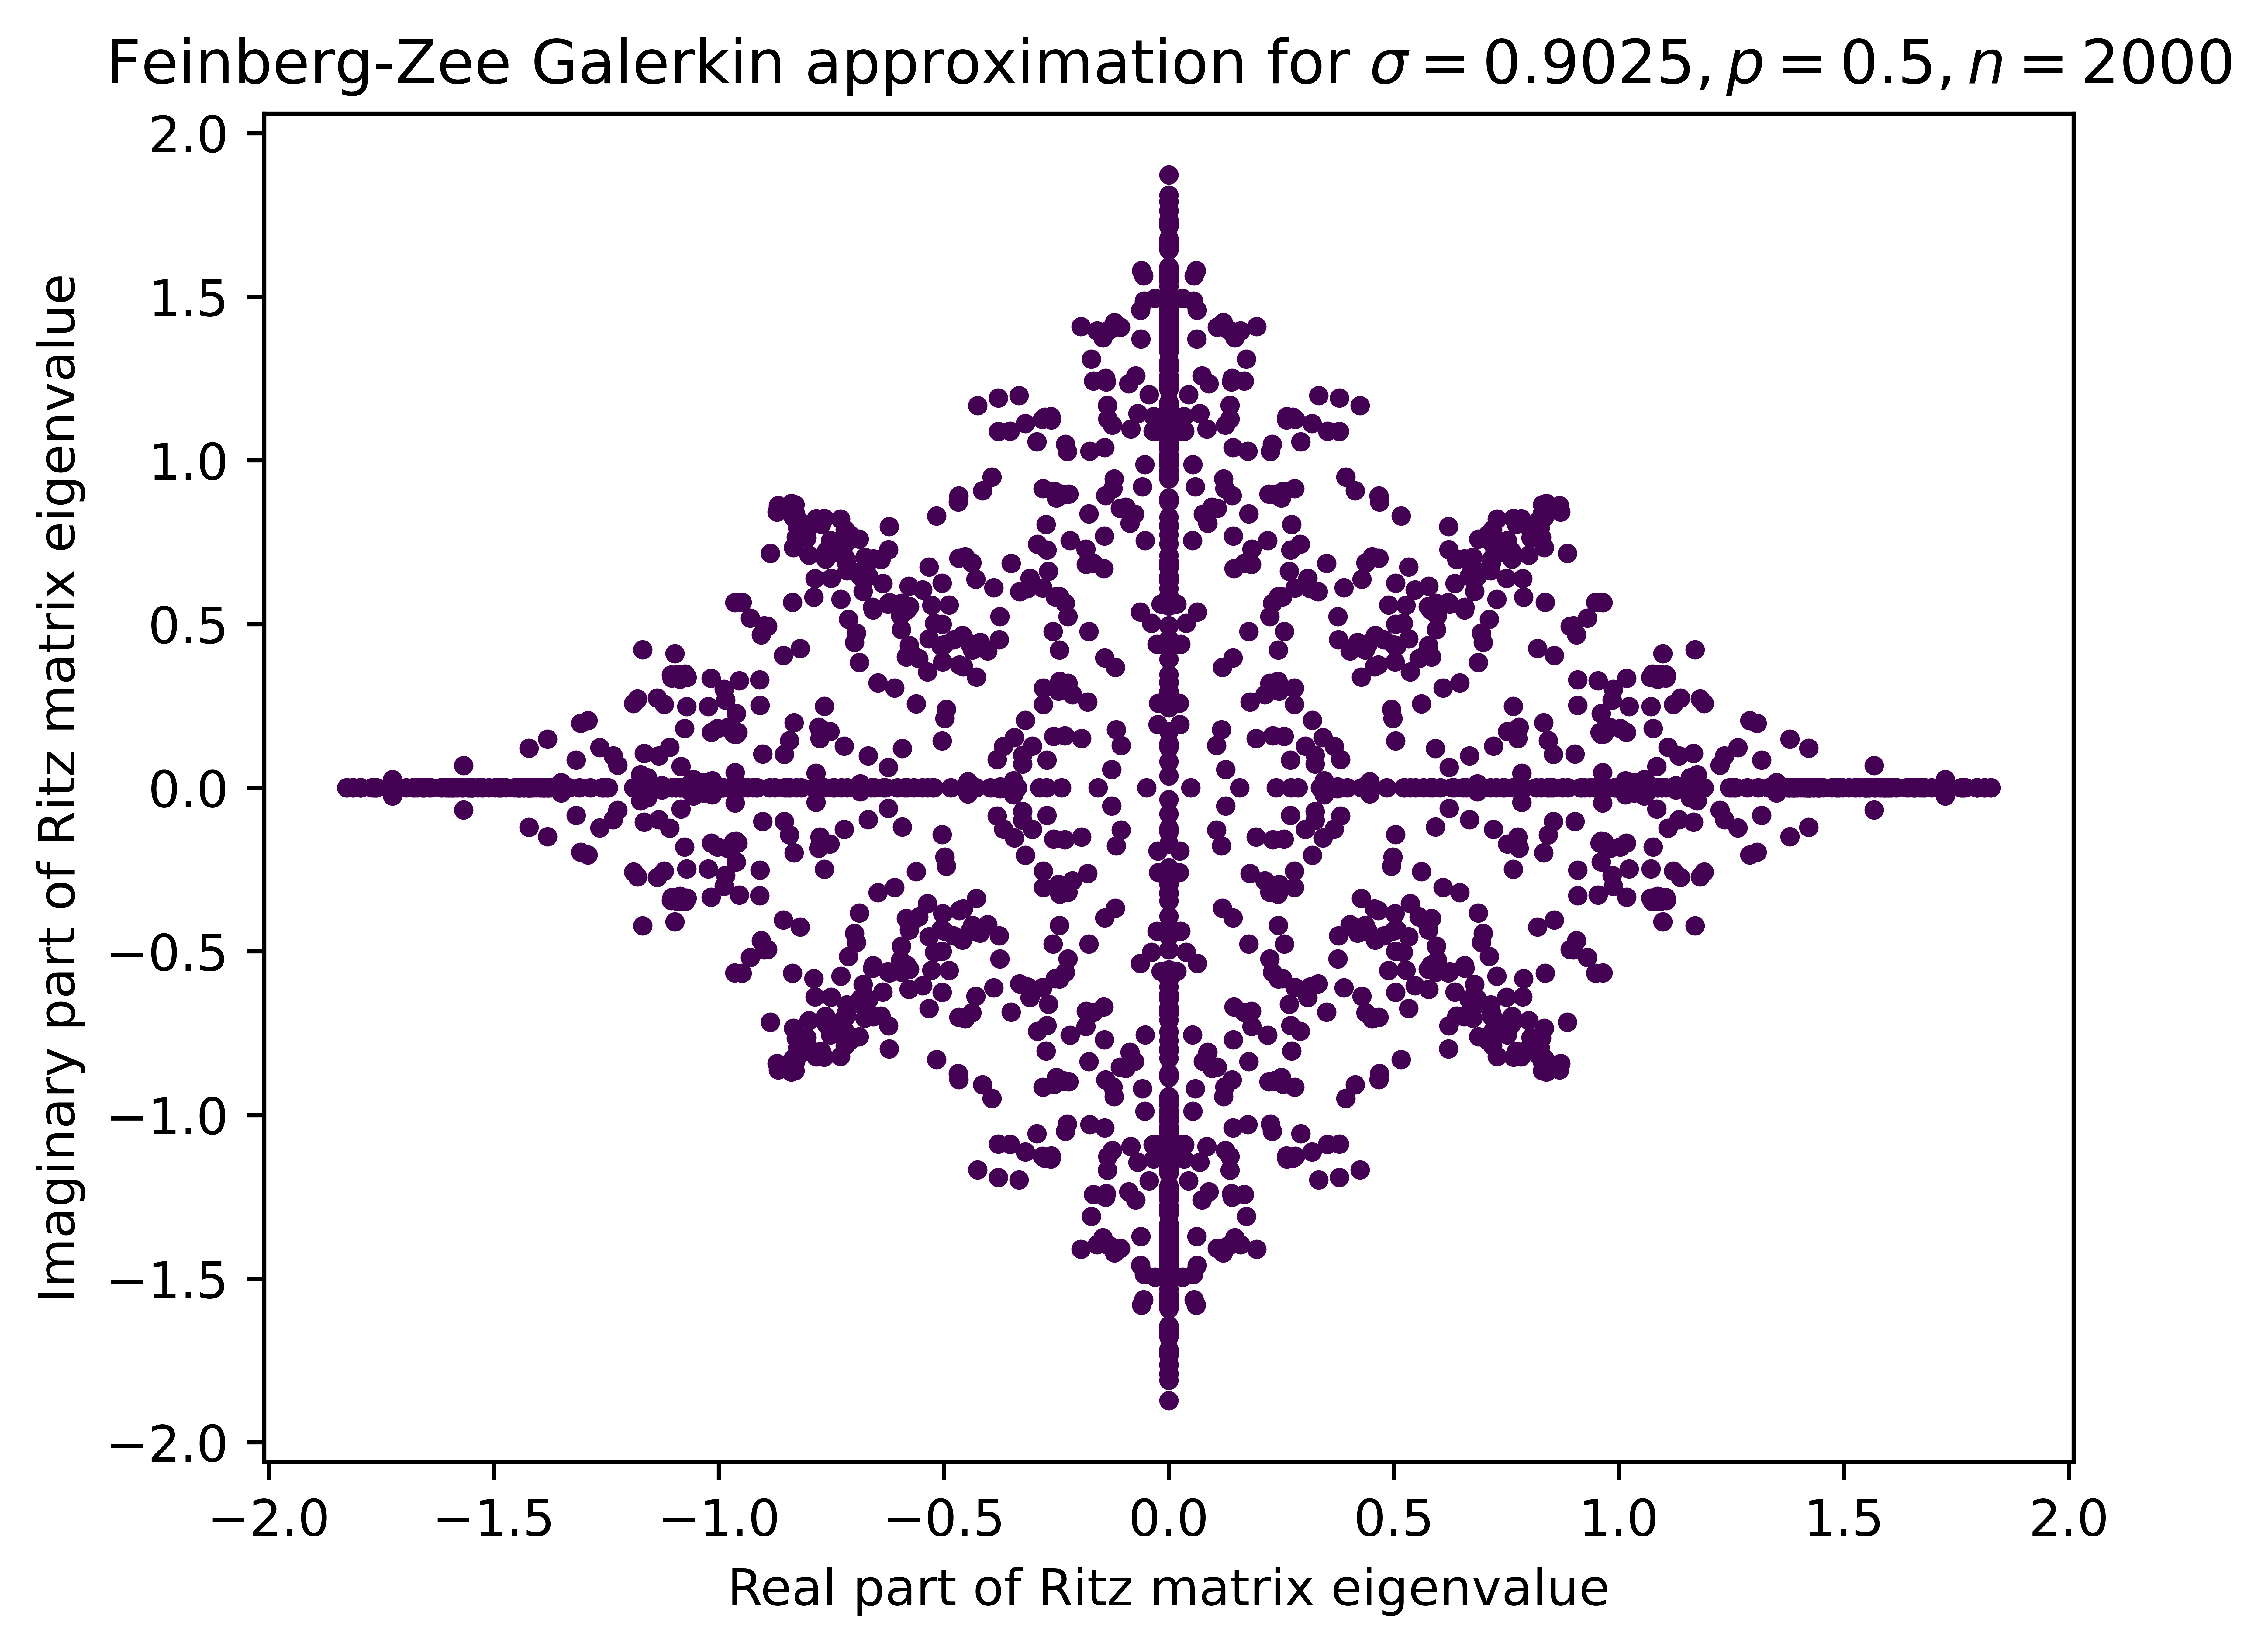
\includegraphics[width=\textwidth]{feinberg-zee-galerkin}
\end{subfigure}
\begin{subfigure}{0.4\textwidth}
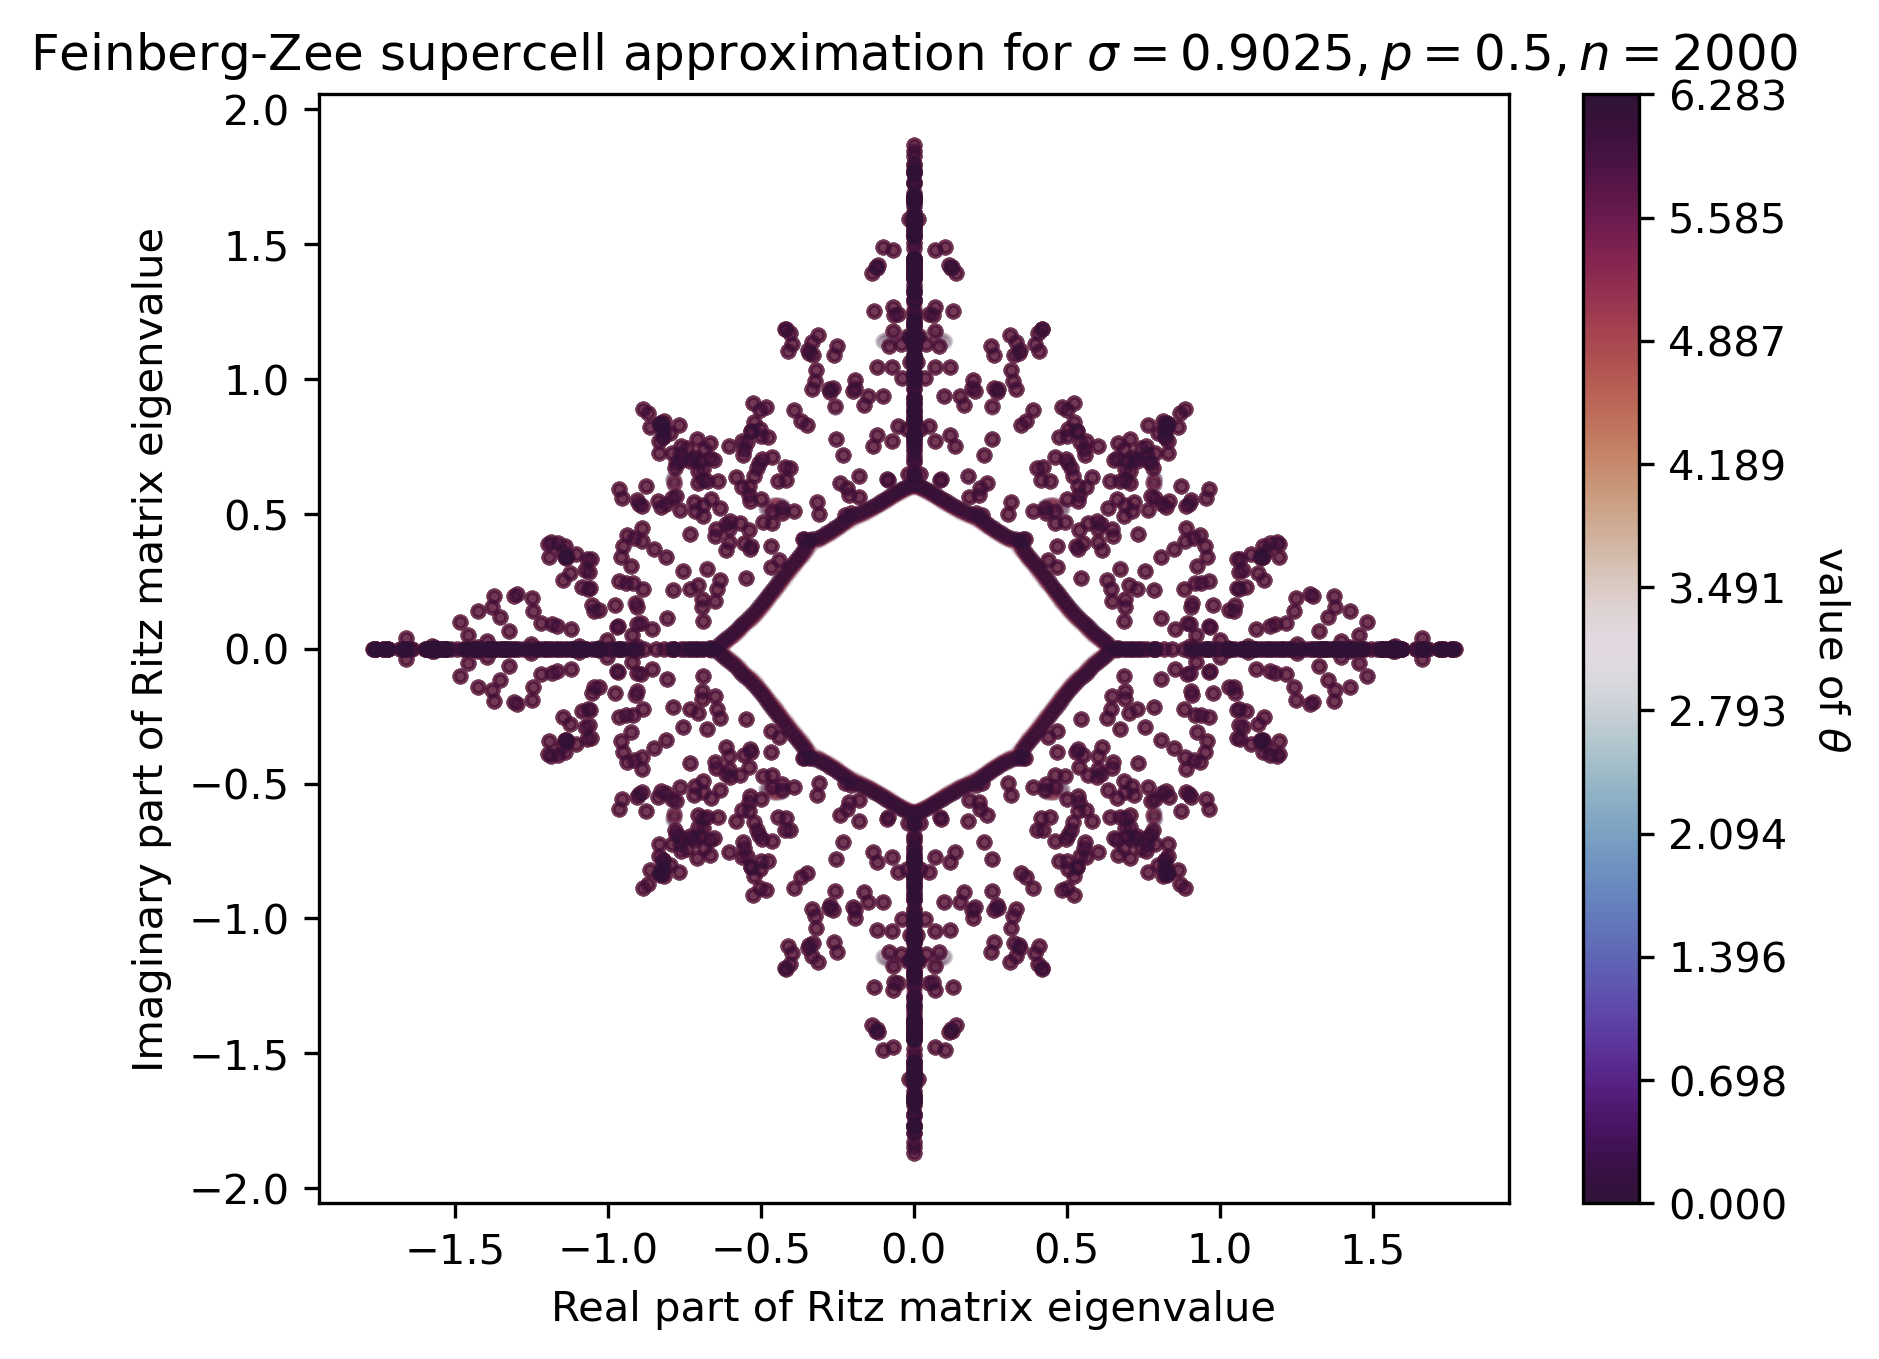
\includegraphics[width=\textwidth]{feinberg-zee-supercell}
\end{subfigure}
\caption{Galerkin and supercell approximations for the Feinberg-Zee operator, with matrix size of 2000. Colour is used on the supercell graph to distinguish different values of $\theta$, which were 50 evenly distributed values between $0$ and $2 \pi$, and the same random sequence was used in both cases. One can see the quite startling difference between the two; the hole in the supercell approximation. Chandler-Wilde and Davies \cite{chandler-wilde2012spectrum} conjecture that this hole is in fact present in the actual spectrum of $A^{per}$, suggesting that the Galerkin approximation is quite far from the truth in this case.}
\end{figure}
\clearpage

\end{document}